\section{Antifragile Learning}

\subsection{What is Antifragile Learning}

Antifragile learning is simply an anti-fragile knowledge generation system. Antifragile learning aims not to reduce the number of mistakes or errors - \textbf{it aims to learn from them}, even if the new found knowledge is about what does not work. Antifragile learning is not concerned about being certain of how things work - \textbf{it's primary focus is on self-correcting as fast as possible towards an increasingly more accurate knowledge base}. Antifragile learning embraces the fact that [knowledge is fragile](knowledge-is-fragile.md).

While knowledge is fragile, the process of improving one's knowledge can be made to be antifragile! By systematically improving our understanding of how a system works by both via negativa (what does not work) and via positiva (what seems to work) - while leaving the door open for refutation to come in and prove us wrong.

\subsection{What is unique about this approach}

\textbf{Antifragile learning creates a stark contrast with how the education system works and, notoriously, how modern scientific research works}, especially if said research is heavily sponsored by profit oriented companies and organizations looking to find evidence that their products work by doing no harm (looking for evidence of absense!). More on this in the chapter about Scientism.

The education system and scientific research is very linear (and fragile) because their primary focus is summarized by:
\begin{enumerate}
	\item The less mistakes you make, the better you are.
	\item Learning is about recalling answers to known problems.
	\item Focus on being right (confirmation bias).
\end{enumerate}


Antifragile learning or, better yet, antifragile knowledge generation systems are the polar opposite:
\begin{enumerate}
	\item It welcomes mistakes because they are a source of not only confirmation that something doesn't work but also a source of unexpected solutions to problems we were not necessarily looking to solve.
	\item Learning is about seeking answers to new, unknown, and often unexpected problems.
	\item Focus on systematically improving our knowledge base.
\end{enumerate}


\subsection{Seeking Truth Over Being Right}

In the pursuit of scientific progress, the goal is not to be right. The goal is to uncover truth — especially the inconvenient or uncomfortable kind.

This chapter introduces antifragile learning, a framework where errors are not only tolerated but essential. Systems that improve when stressed — that benefit from disorder — are antifragile. A scientific system built around this principle must embrace, expose, and even reward its own mistakes. Every failure in science is a potential contribution. Yet, a culture of perfectionism persists: researchers polish their papers, hide their mistakes, and present their results as flawless. This does not reflect reality. No system is perfect. Every theory has edge cases. Every experiment contains assumptions that may not hold across all contexts. To make genuine progress, we must surface errors. Especially in cases where a theory breaks down despite overwhelming evidence of its general correctness. Science advances not by confirming what already works, but by revealing where it doesn't.

\subsection{The Asymmetry of Failure and the Problem of Ruin}

Not all failures are equal. 

Some errors are recoverable. Others — especially when scaled — lead to ruin, a catastrophic, irreversible outcome.

This means that we can't just think about ruin in an isolated way. We need to consider what is the cost of being wrong because, chances are, we might be wrong at along.

\subsubsection{The Cost Of Being Wrong}
To evaluate this risk, we must ask ourservels:

\begin{itemize}
	\item \textbf{What is the scale of ruin?} Does the failure impact one person or millions?
	\item \textbf{What is the impact of ruin?} Minor inconvenience, or existential threat?
	\item \textbf{What is the complexity of the system involved?} Low-complexity predictive systems (e.g., a bug in a software program responsible for sending emails) fail in predictable ways. High-complexity systems (e.g., human biology, ecosystems) may fail in ways we can’t anticipate.
\end{itemize}

The cost of being wrong in a high-complexity, high-impact context — like a bioengineered drug — is vastly more dangerous than one that fails in a way that just poses a slight annoyance - like a toy breaking up. 

So, let's focus, for now, on high-complexity and non-linear systems. This leaves out 2 variables which are the Scale of Ruin and Impact of Ruin.

\begin{center}
	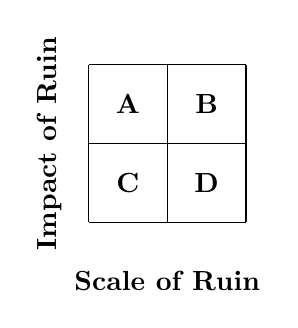
\begin{tikzpicture}
		% Draw grid
		\foreach \x in {0,...,2} {
			\draw (\x, 0) -- (\x, 2);
			\draw (0, \x) -- (2, \x);
		}
		
		% Axis labels
		\node[below] at (1, -0.5) {\textbf{Scale of Ruin}};
		\node[rotate=90] at (-0.5, 1) {\textbf{Impact of Ruin}};
		
		% Cell labels
		\node at (0.5, 1.5) {\textbf{A}};
		\node at (1.5, 1.5) {\textbf{B}};
		\node at (0.5, 0.5) {\textbf{C}};
		\node at (1.5, 0.5) {\textbf{D}};
	\end{tikzpicture}
\end{center}

% Reference list
\begin{enumerate}
	\item (A) \textbf{High Impact, Low Scale:} this affects individuals at a small scale. An example here would be you being poisoned by your worst enemy. The ruin impact will be high... for you.
	\item (B) \textbf{High Impact, High Scale}: this is the worst case scenario. The ruin impact here is high and it's at a high scale, so think, in an extreme case, annihilation at a global scale, say, a nuclear war.
	\item (C) \textbf{Small Impact, Small Scale}: lowest risk possible... impacting only a few individuals.
	\item (D) \textbf{Small Impact, High Scale}: here the impact is small but it affects a lot of people... so caution is advised.
\end{enumerate}

To be clear - we're not prescribing what to do when you are dealing with each of the scenarios of ruin above. All we're trying to do is bring awareness of what quadrant you're in so you can behave accordingly.

\subsubsection{Ruin Exposure as an Innovation Driver}

Not all is bad when we talk about ruin though... Ruin exposure introduces an unexpected twist that is frequently ignored, which is how ruin can be an incredibly powerful driver for innovation. 

Think about this - what is one of the greatest ruin threats to Humanity? War. For centuries, war has been used as an innovation driver to develop advanced technology that can either reduce a country's ruin exposure or increase the threat of ruin to others.

Here's some examples:

\textbf{Cryptography and the Birth of Modern Computing}
\begin{itemize}
	\item \textbf{Innovation}: Colossus (1944) – The first programmable digital electronic computer.
	\item \textbf{Context}: British codebreakers at Bletchley Park, led by Alan Turing and others, built Colossus to break the German Lorenz cipher.
	\item \textbf{Impact}: Demonstrated the power of automation and programmable logic, inspiring later stored-program computers. \cite{colossus2006}
\end{itemize}

\textbf{Ballistics and Numerical Computation}
\begin{itemize}
	\item \textbf{Innovation}: ENIAC (1945) – Electronic Numerical Integrator and Computer.
	\item \textbf{Context}: Designed by the U.S. Army for calculating artillery firing tables.
	\item \textbf{Impact}: First general-purpose electronic computer. Influenced the development of modern computing architectures. \cite{montecarlo2014}
\end{itemize}

\textbf{Radar and Real-Time Signal Processing}
\begin{itemize}
	\item \textbf{Innovation:} Real-time computing, analog-to-digital conversion.
	\item \textbf{Context}: British and American radar development during WWII.
	\item \textbf{Impact}: Led to signal processing methods foundational to modern communications, audio/video tech, and sensor data interpretation. \cite{Whirlwind1980}
\end{itemize}

\textbf{Nuclear Weapons and Simulation}
\begin{itemize}
	\item \textbf{Innovation}: Monte Carlo simulations, large-scale numeric simulations.
	\item \textbf{Context}: Developed at Los Alamos to model nuclear reactions (e.g., Manhattan Project).
	\item \textbf{Impact}: Core methodology in modern computing—from climate models to AI training \cite{MonteCarloMethod1949}
\end{itemize}

\textbf{Communications and Networking}
\begin{itemize}
	\item \textbf{Innovation}: Packet switching and ARPANET (precursor to the Internet).
	\item \textbf{Context}: Cold War concern over nuclear survivability of communications.
	\item \textbf{Impact}: DARPA-funded research led to resilient, decentralized networking—foundational to the Internet. \cite{Leiner2009}
\end{itemize}

\textbf{Solid-State Electronics}
\begin{itemize}
	\item \textbf{Innovation}: Transistors (1947) and integrated circuits (1950s–60s).
	\item \textbf{Context}: Cold War race for lighter, faster, more durable tech (e.g., for missiles and space).
	\item \textbf{Impact}: Enabled the transition from room-sized machines to personal computers and mobile tech. \cite{RiordanHoddeson1997}
\end{itemize}

\textbf{Satellite and GPS Technology}
\begin{itemize}
	\item \textbf{Innovation}: Global Positioning System (GPS).
	\item \textbf{Context}: Cold War-era navigation systems for ballistic missiles and aircraft.
	\item \textbf{Impact}: Now central to navigation, mapping, mobile apps, and more. \cite{Pace1995}
\end{itemize}

\textbf{Surveillance and Image Processing}
\begin{itemize}
	\item \textbf{Innovation}: Remote sensing, real-time video and pattern recognition.
	\item \textbf{Context}: Reconnaissance satellites, drone technology, signal intelligence.
	\item \textbf{Impact}: Advanced imaging, video compression, and early computer vision systems. \cite{Krick1971}
\end{itemize}

\subsection{Black Swans and the Fragility of Knowledge}

It only takes one black swan to disprove the claim that “all swans are white.” Likewise, it takes only one refuting case to falsify a scientific theory. Thus, the most valuable scientific contributions may not be those that reinforce existing knowledge, but those that break it. For this reason, knowledge should always be open to be challenged, always tentative in its conclusions. The higher the cost of being wrong, the more important it is to stress-test it.

Antifragile learning does not fear the fragility of errors and mistakes in our knowledge. It wants to expose them and learn from them!

\subsection{Not all research is created equal}

The scientific knowledge being generated needs to be assessed based on:
\begin{itemize}
	\item The exposure to ruin if the claim is wrong.
	\item The complexity of the system in which it operates.
	\item The number of people affected by its failure.
\end{itemize}

This gives us a heuristic: prioritize scrutiny for high-risk, high-scale, high-complexity claims — especially those promoted by actors with no downside.

\subsection{The Cost of Being Wrong}

In antifragile learning, the goal is not to avoid being wrong — because that’s impossible — but to understand the cost of being wrong.

Mistakes happen. Being wrong is inevitable, especially in the exploration of complex systems. But not all errors are equal. Some are cheap. Others can be catastrophic. 

The critical insight is this:
\begin{quote}
	We do not fear errors by themselves. We fear the cost of errors.
\end{quote}

When scientists, engineers, or policymakers make decisions, they must assess not just the probability of something go wrong — but what happens if 
it does go wrong. This is especially true in high-stakes domains like medicine, AI safety, climate systems, and synthetic biology.

This leads us to a vital principle in antifragile thinking: \textbf{The greater the cost of being wrong, the more we must stress-test the claim.}

Errors and mistakes can't be evaluated in a vacuum. We need to understand what is the cost of being wrong. 

We need to evaluate the exposure to ruin in several dimensions:

\begin{itemize}
	\item \textbf{Scale}: what is the scale of the exposure to ruin? From the micro level (individual) to the macro level (entire populations)
	\item \textbf{Impact}: what is the severity of the impact? From low-impact (people get sick) to high-impact (people die)
	\item \textbf{Complexity}: what is the level of complexity of the target system? From low complexity (linear systems) to high complexity (non-linear systems)
\end{itemize}

We will focus on high complexity systems only, so that leaves us with \textit{scale} and \textit{impact} to be measured.
If you plot a 4x4 matrix, you will quickly realize that the top right quadrant is the most dangerous and, thus, the one we must be most prepared for: high scale and high impact errors.

Even worse is when the cost of being wrong doesn't fall on the person making the claim. This is where skin in the game becomes essential. If I claim a biotech intervention is safe, but am not exposed to its possible failure — and others are — then I am transferring the cost of being wrong to them. That is unacceptable in an antifragile system.

\section{Scientism is not Science!}
Ultimately, with this platform, we want to end the Scientism which is heavily based on scientific research being sponsored by for profit companies and organizations.

Production of confirmation in service of profit is not science - it is Scientism — a dogmatic belief in science-like signals (e.g., peer-reviewed publications, institutional consensus, statistical significance) as inherently trustworthy, while ignoring the structure of incentives behind them and silencing dissenting voices and research that refutes them.

\subsection{Iatrogenisis or Iatrogenics}

``Medicine has known about iatrogenics since at least the 4th century before our era - \emph{primum non nocere} (first to no harm) is a first principle attributed to Hippocrates and integrated in the so-called Hippocratic Oath taken by every medical doctor on his commencement day.''\cite{Taleb2012}

In spite of that fact, there is ample evidence of multiple cases of Iatrogenisis. \cite{VarleyVarma2021}

Here's some examples:

\subsubsection{Ignaz Semmelweis and Handwashing}

In the mid-19th century, Ignaz Semmelweis, a Hungarian physician, noticed that the mortality rate of women giving birth in hospitals was significantly higher than those attended by midwives at home. He suspected that  ``childbed fever'' (puerperal fever) was being transmitted by doctors who were not washing their hands after performing autopsies and before delivering babies.

Despite evidence supporting his theory, the medical community largely rejected his ideas. It took years for the concept of handwashing to be widely accepted and for proper hygiene practices to be adopted, eventually leading to a significant reduction in infections.

References: \cite{Semmelweis2006}

\subsubsection{Thalidomide}
In the late 1950s and early 1960s, thalidomide was a drug prescribed to pregnant women to alleviate morning sickness. However, it was later discovered that the drug caused severe birth defects, especially
limb deformities, in newborns. The tragic outcome of thalidomide use highlighted the importance of rigorous testing for drug safety, especially during pregnancy, and led to significant changes in drug
regulation and testing protocols.

References: \cite{WGMcbride}

\subsubsection{Diethylstilbestrol}
Diethylstilbestrol was prescribed to pregnant women from the 1940s to the early 1970s to prevent miscarriages and complications during pregnancy. Decades later, it was found that daughters of these women
had a higher risk of developing reproductive tract abnormalities and a rare form of vaginal cancer.

References: \cite{Diethylstilbestrol2000}

\subsubsection{Fen-Phen}
Fen-Phen was a combination of two drugs, fenfluramine and phentermine, prescribed for weight loss in the 1990s. It was later discovered that fenfluramine could cause serious heart valve problems and primary
pulmonary hypertension, leading to the withdrawal of the drug from the market.

References: \cite{Wolff1997}

\subsubsection{The polio vaccine (IPV) and The Cutter Incident in 1955}

In April 1955 more than 200 000 children in five Western and mid-Western USA states received a polio vaccine in which the process of inactivating the live virus proved to be defective. Within days there were reports of paralysis and within a month the first mass vaccination programme against polio had to be abandoned. Subsequent investigations revealed that the vaccine, manufactured by the California-based family firm of Cutter Laboratories, had caused 40 000 cases of polio, leaving 200 children with varying degrees of paralysis and killing 10.

References: \cite{Fitzpatrick2006}

\subsection{Scientific Absolutism Powered by Capitalism}

\subsubsection{The Opioid Epidemic – Purdue Pharma and the Illusion of Safety}

Purdue Pharma aggressively marketed OxyContin as a safe, non-addictive painkiller, citing selectively crafted studies and physician testimonials. Internally, however, the company knew about the drug's addictive potential. It used industry-funded research, manipulated scientific claims, and influenced medical guidelines to downplay harm.

By the time the truth surfaced, the damage was massive. Over 500,000 deaths from opioid overdoses in the U.S. alone, an entire generation affected by addiction and billions in healthcare and social costs.

The cost of being wrong was catastrophic — and largely externalized. Purdue paid fines, but executives faced minimal consequences. The system had no skin in the game.

\cite{CBSnewsPurduePharma}
\cite{PBSPurduePharma}
\cite{Alonso2021}

\subsubsection{Glyphosate and Monsanto – “No Evidence of Harm” as a Weapon}

Monsanto, now part of Bayer, developed glyphosate (marketed as Roundup) and ensured its widespread use in global agriculture. For years, Monsanto-funded studies claimed there was “no evidence” that glyphosate was carcinogenic.

But this consensus was shaped by ghostwriting studies that appeared independent but were actually drafted by Monsanto; suppressing dissenting research and attacking independent scientists who raised concerns.

In 2015, the World Health Organization’s International Agency for Research on Cancer (IARC) classified glyphosate as "probably carcinogenic to humans." Thousands of lawsuits followed, and Bayer has since 
paid billions in settlements.

This case exemplifies how scientific absolutism, powered by capital, can become a shield for harm. Consensus was not evidence of truth — it was the product of sustained influence.

\cite{GLENNA2021104290}
\cite{mindthegap2020}
\cite{ehn2018}

\subsubsection{Theranos – The Cult of Proof Without Validation}

Theranos, the biotech startup founded by Elizabeth Holmes, promised revolutionary blood testing using a
single drop of blood. Investors, media, and even regulatory bodies were convinced — not by open
peer-reviewed research, but by carefully curated internal “proof”.

Behind the scenes devices didn't work, test results were unreliable and potentially dangerous and employees who spoke out were silenced or retaliated against.

Theranos thrived in a system where credibility was built through branding and controlled narratives, not 
scientific falsifiability. It wasn't until whistleblowers and investigative journalists exposed the fraud
that the collapse occurred.

Theranos shows what happens when the appearance of science is weaponized — and when those in charge face
zero downside if they’re wrong.

\cite{USvsHolmes2022}
\cite{buzzfeednews2018}
\cite{justivegove-theranos}

\subsection{To sum it up}

When capitalism fuels science with no guardrails, it creates deep epistemic risks:
\begin{itemize}
	\item \textbf{Funders seek positive results}: They want validation that the drug is safe, the product works, the chemical poses no harm.
	\item \textbf{Researchers are subtly incentivized}: Careers, grants, promotions, and publications depend on "publishable" results — often meaning confirmation, not contradiction.
	\item \textbf{Negative results are buried}: Data showing harm, inefficacy, or contradictions are quietly omitted, downplayed, or never published at all.
\end{itemize}

This creates a fragile body of “knowledge” — one that appears robust but collapses under adversarial scrutiny. Not so with us!  This capitalist-scientific complex promotes a false sense of certainty. A new drug is approved because “studies show it’s safe”. A pesticide is used worldwide because “there’s no evidence of harm”. An AI system is deployed because “tests show it sounds safe”. But the absence of evidence is not the evidence of absence. 

When dissenting results are suppressed or never surfaced, the consensus becomes a lie of omission. The cost? Long-term systemic harm — to human bodies, ecological systems, and societal trust in science itself.

The only way out is to realign scientific practice with antifragile principles:
\begin{itemize}
	\item \textbf{Open adversarial testing}: Allow and reward attempts to falsify claims.
	\item \textbf{Transparency of funding and incentives}: Make biases visible, not hidden.
	\item \textbf{Permanent record of disproofs}: Not just what was found to work, but what was proven not to work — and why.
	\item \textbf{Distributed credibility}: Don’t centralize truth around institutions, but around reproducibility and resistance to critique.
\end{itemize}